\chapter{认识你的电脑}
\label{cha:computer-and-its-components}

\begin{intro}
  或许电脑对你来说,是一个熟悉却又神秘的「黑箱」:它早已融入我们的生活,但我们却很少真正了解它的组成与结构。阅读完本章,你将找到这些问题的答案:

  \begin{itemize}
    \item 什么是「CPU」?别人说的「i5」「i7」都是什么?「双核」「四核」又是什么?
    \item 为什么说「内存」和「硬盘」不一样?存储东西的到底是内存还是硬盘?电脑特别卡,到底是内存不够还是硬盘不够?
    \item 我想玩游戏,选购电脑时应该关注什么方面?「显卡」是什么东西?
    \item 什么是「Windows」?那「Windows 11」又是什么?为什么苹果笔记本的系统界面看起来和我不一样?我用的是什么系统?
  \end{itemize}
\end{intro}

如今,电脑几乎「无所不能」,已经成为了我们生活和工作中不可或缺的一部分。每一台电脑内部,都充满了复杂的电子电路和元器件,它们是人类智慧的结晶,构成了电脑的「硬件」部分。而在这冷冰冰的硬件之上,「软件」赋予了电脑生命与功能——从办公、学习到娱乐,各种软件让我们的生活更加便捷。可以说,硬件如同电脑的「身体」,软件则是电脑的「思维」,它们共同构成了「电脑」这个有机体。

本章将引领你深入认识自己的电脑:从最基础的硬件开始,我们将逐一介绍它们的功能与作用,并分析这些硬件如何影响电脑的性能。接着,我们将了解运行在这些硬件之上的各种软件,介绍它们与硬件的协同和配合,让你对电脑的构成和运行有一个更加全面的了解。

\section{电脑内部的硬件} 

本节我们将介绍电脑内部的那些关键硬件。即使你并没有亲眼见过各种硬件模块的模样,但通过这一节的介绍,你也会对它们形成基本的了解。

在开始之前,我们先假设这样一个场景:某位老师收集了一个班的作业,现在需要批改它们,如下图所示。

\begin{figure}[htb!]
  \centering
  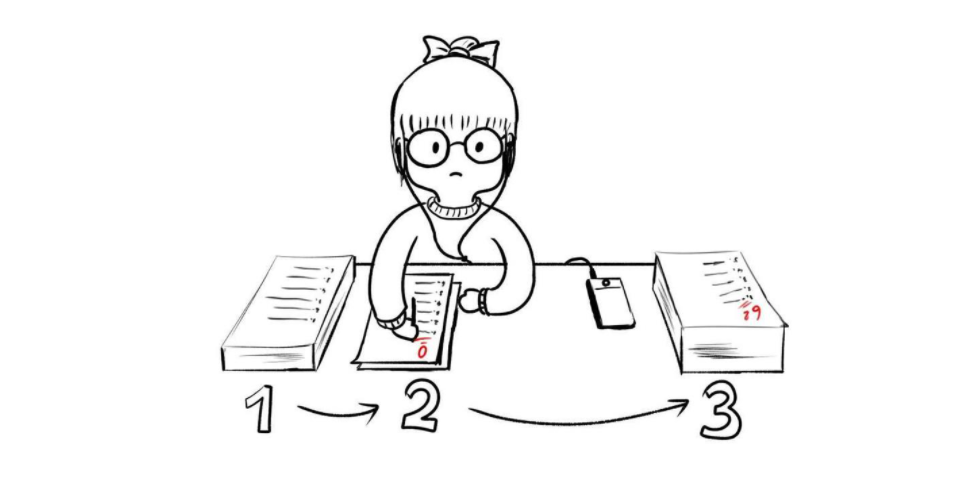
\includegraphics[width=.5\textwidth]{assets/basic/Teacher_and_homework.png}
  \caption{正在批改作业的老师}
  \label{fig:teacher-and-homework}
\end{figure}

我们可以把老师批改作业的过程分解成下面的步骤:

\begin{enumerate}
  \item 老师将这一摞作业堆在办公桌的一边,腾出办公桌的中央和另一边。
  \item 现在,老师取下这一摞作业中的一小叠,放在办公桌中央,开始伏案批改。
  \item 老师批改完了这一小叠作业,然后将它们放在办公桌的另一边,摞成新的一沓。
  \item 重复步骤 2 和步骤 3,最终老师完成了全部作业的批改,这时批改完的作业全部在办公桌的另一边。
\end{enumerate}

这个例子有什么用呢?请先记住它,它将帮助我们更好地理解电脑硬件的工作原理。

\subsection{处理器(CPU)}

中央处理器(Central Processing Unit),简称「处理器」,英文简写「CPU」,是电脑内部最重要的一枚芯片,可以想象成是电脑的「大脑」。在上面的例子中,老师就相当于电脑中的处理器:老师的作用是批改作业,从而完成教学任务;处理器的作用是进行各种运算,从而实现电脑不同的功能。

你一定注意到过,电脑会发热——热到需要用一个风扇给它降温,这热量中有很大一部分就是处理器发出来的。如果你有关注过时事和新闻,中美贸易战之中关键的一环,正是处理器芯片。下图中,左边是一枚台式机的 CPU,右边是一枚笔记本电脑的 CPU。

\begin{figure}[htb!]
  \centering
  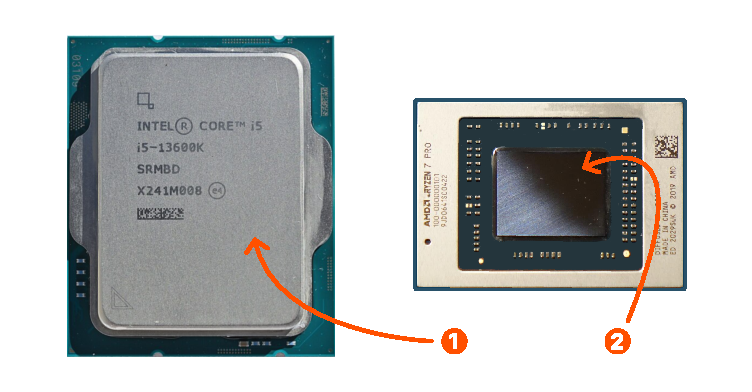
\includegraphics[width=.6\textwidth]{assets/basic/Two_CPUs.pdf}
  \caption{常见的台式机和笔记本电脑的处理器芯片}
  \label{fig:Two_CPUs}
\end{figure}

\begin{note}
  你可能会疑惑:这两个 CPU 为什么看起来很不一样?这是因为笔记本 CPU 为了节省空间,会直接将 \underline{➋「晶片」}(芯片的核心部分,由硅制成)裸露在外;而台式机 CPU 为了保护晶片,会在其外罩上一层 \underline{➊ 金属盖}。
\end{note}

处理器是电脑工作的核心,因此,\regcolor{处理器的性能就很大程度上决定了电脑的性能,决定了我们使用这台电脑流不流畅、玩游戏卡不卡、工作效率高不高}。在今天,全世界电脑芯片基本上是由两家美国公司设计\footnote{事实上,芯片的「设计」和「制造」两件事是不一样的,就像能设计出房屋的建筑师不一定会到工地上去砌墙。英特尔能够自行完成从设计到制造整条生产链,而 AMD 只能完成设计,它的处理器是由专门负责制造芯片的厂商(例如台积电)生产的。}的,其中一家叫做「英特尔」(Intel),另一家叫做「AMD」。

\begin{itemize}
  \item 英特尔公司现在主要的 CPU 产品线称作「酷睿」(Core),而「酷睿」系列又分成了三个子系列,每个子系列都有不同档次的产品。
    \begin{table}[htb!]
      \centering
      \caption{英特尔CPU产品系列}
      \label{tab:Intel-CPUs}
      \begin{tblr}{
        colspec = XX[2]X[4]X[4],
        cells = {c, m},
        cell{Z}{2-Z} = {j},
        row{1} = {fg = white, bg = missing, font = \bfseries},
        row{even} = {MissingSkyBlue},
      }
        \toprule
        & 传统酷睿系列 & 酷睿 Ultra 系列 & 酷睿数字系列 \\
        \midrule
        低端 & 酷睿 i3 & 酷睿 Ultra 3 & 酷睿 3 \\
        中端 & 酷睿 i5 & 酷睿 Ultra 5 & 酷睿 5 \\
        高端 & 酷睿 i7 & 酷睿 Ultra 7 & 酷睿 7 \\
        顶尖 & 酷睿 i9 & 酷睿 Ultra 9 &  ---\footnotemark \\
        说明 & 传统的酷睿系列,自 2008 年起沿用至今 & 2023 年发布的新系列,主要应用在高端笔记本电脑产品上,增加了针对 AI 应用的优化 & 2024 年发布的新系列,针对笔记本电脑产品进行了能耗方面的优化 \\
        \bottomrule
      \end{tblr}
    \end{table}
    \footnotetext{截至 2024 年 12 月,英特尔并没有推出酷睿 9 系列的 CPU。}\\
    大多数使用英特尔 CPU 的电脑,机器表面会贴一个类似左下图的蓝色(或灰色、黑色)贴纸。对于笔记本电脑,通常贴在键盘下方或机器背面;而对于品牌台式机,则通常贴在机器正面、侧面或顶面,如右下图所示。
    \begin{figure}[htb!]
      \centering
      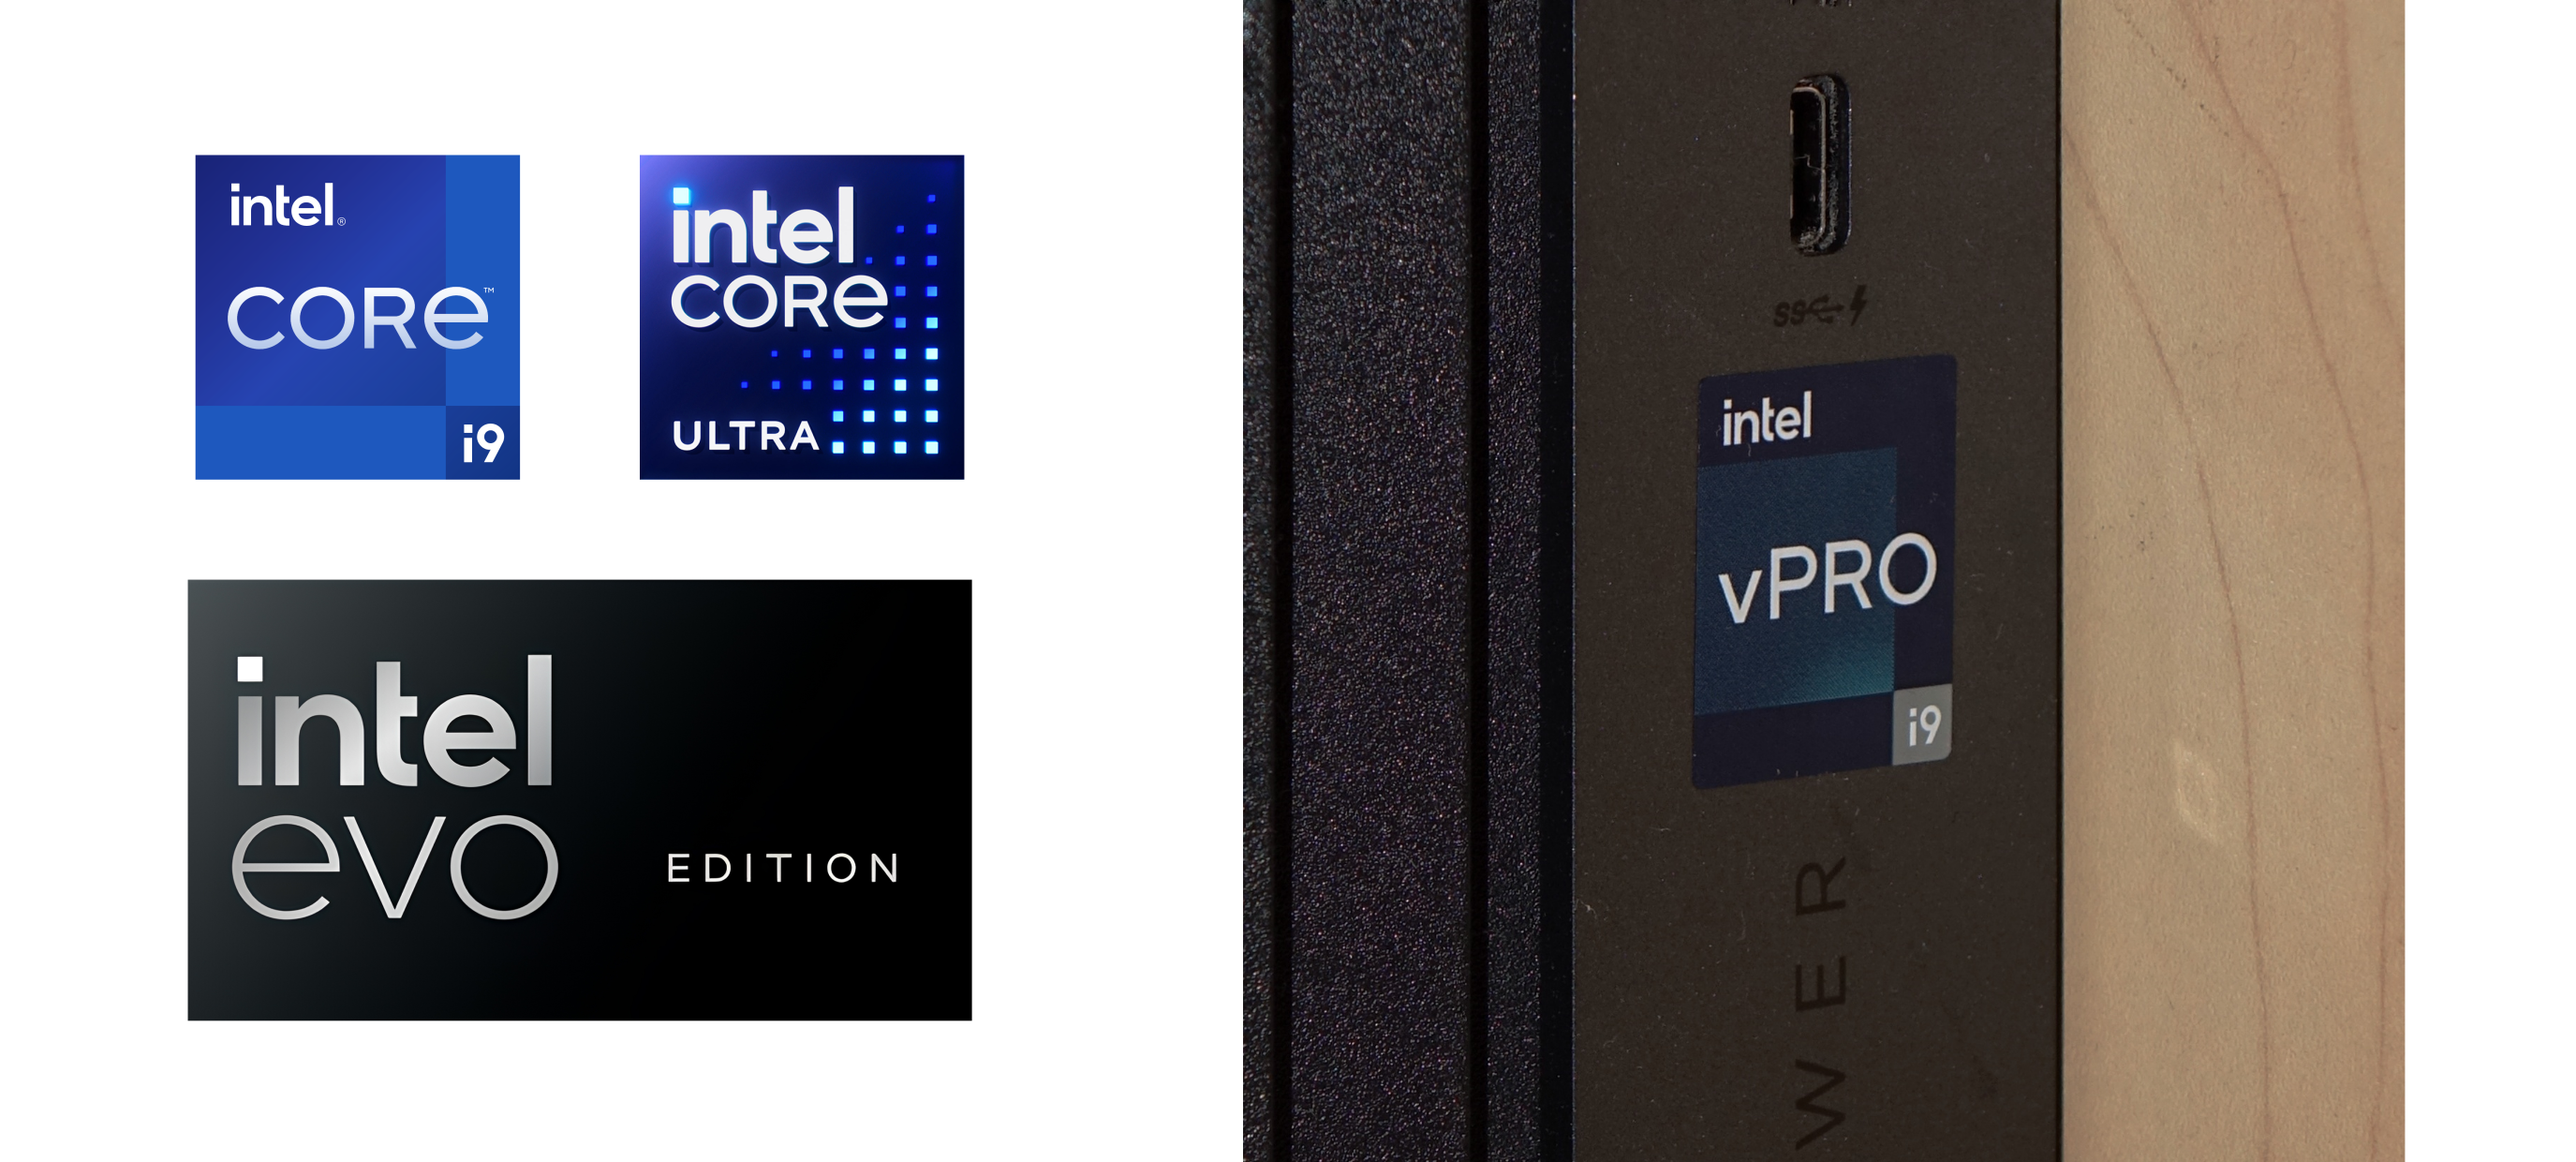
\includegraphics[width=.7\textwidth]{assets/basic/Intel_sticker.png}
      \caption{英特尔的贴纸}
      \label{fig:Intel_sticker}
    \end{figure}\\
    \begin{figure}[htb!]
      \centering
      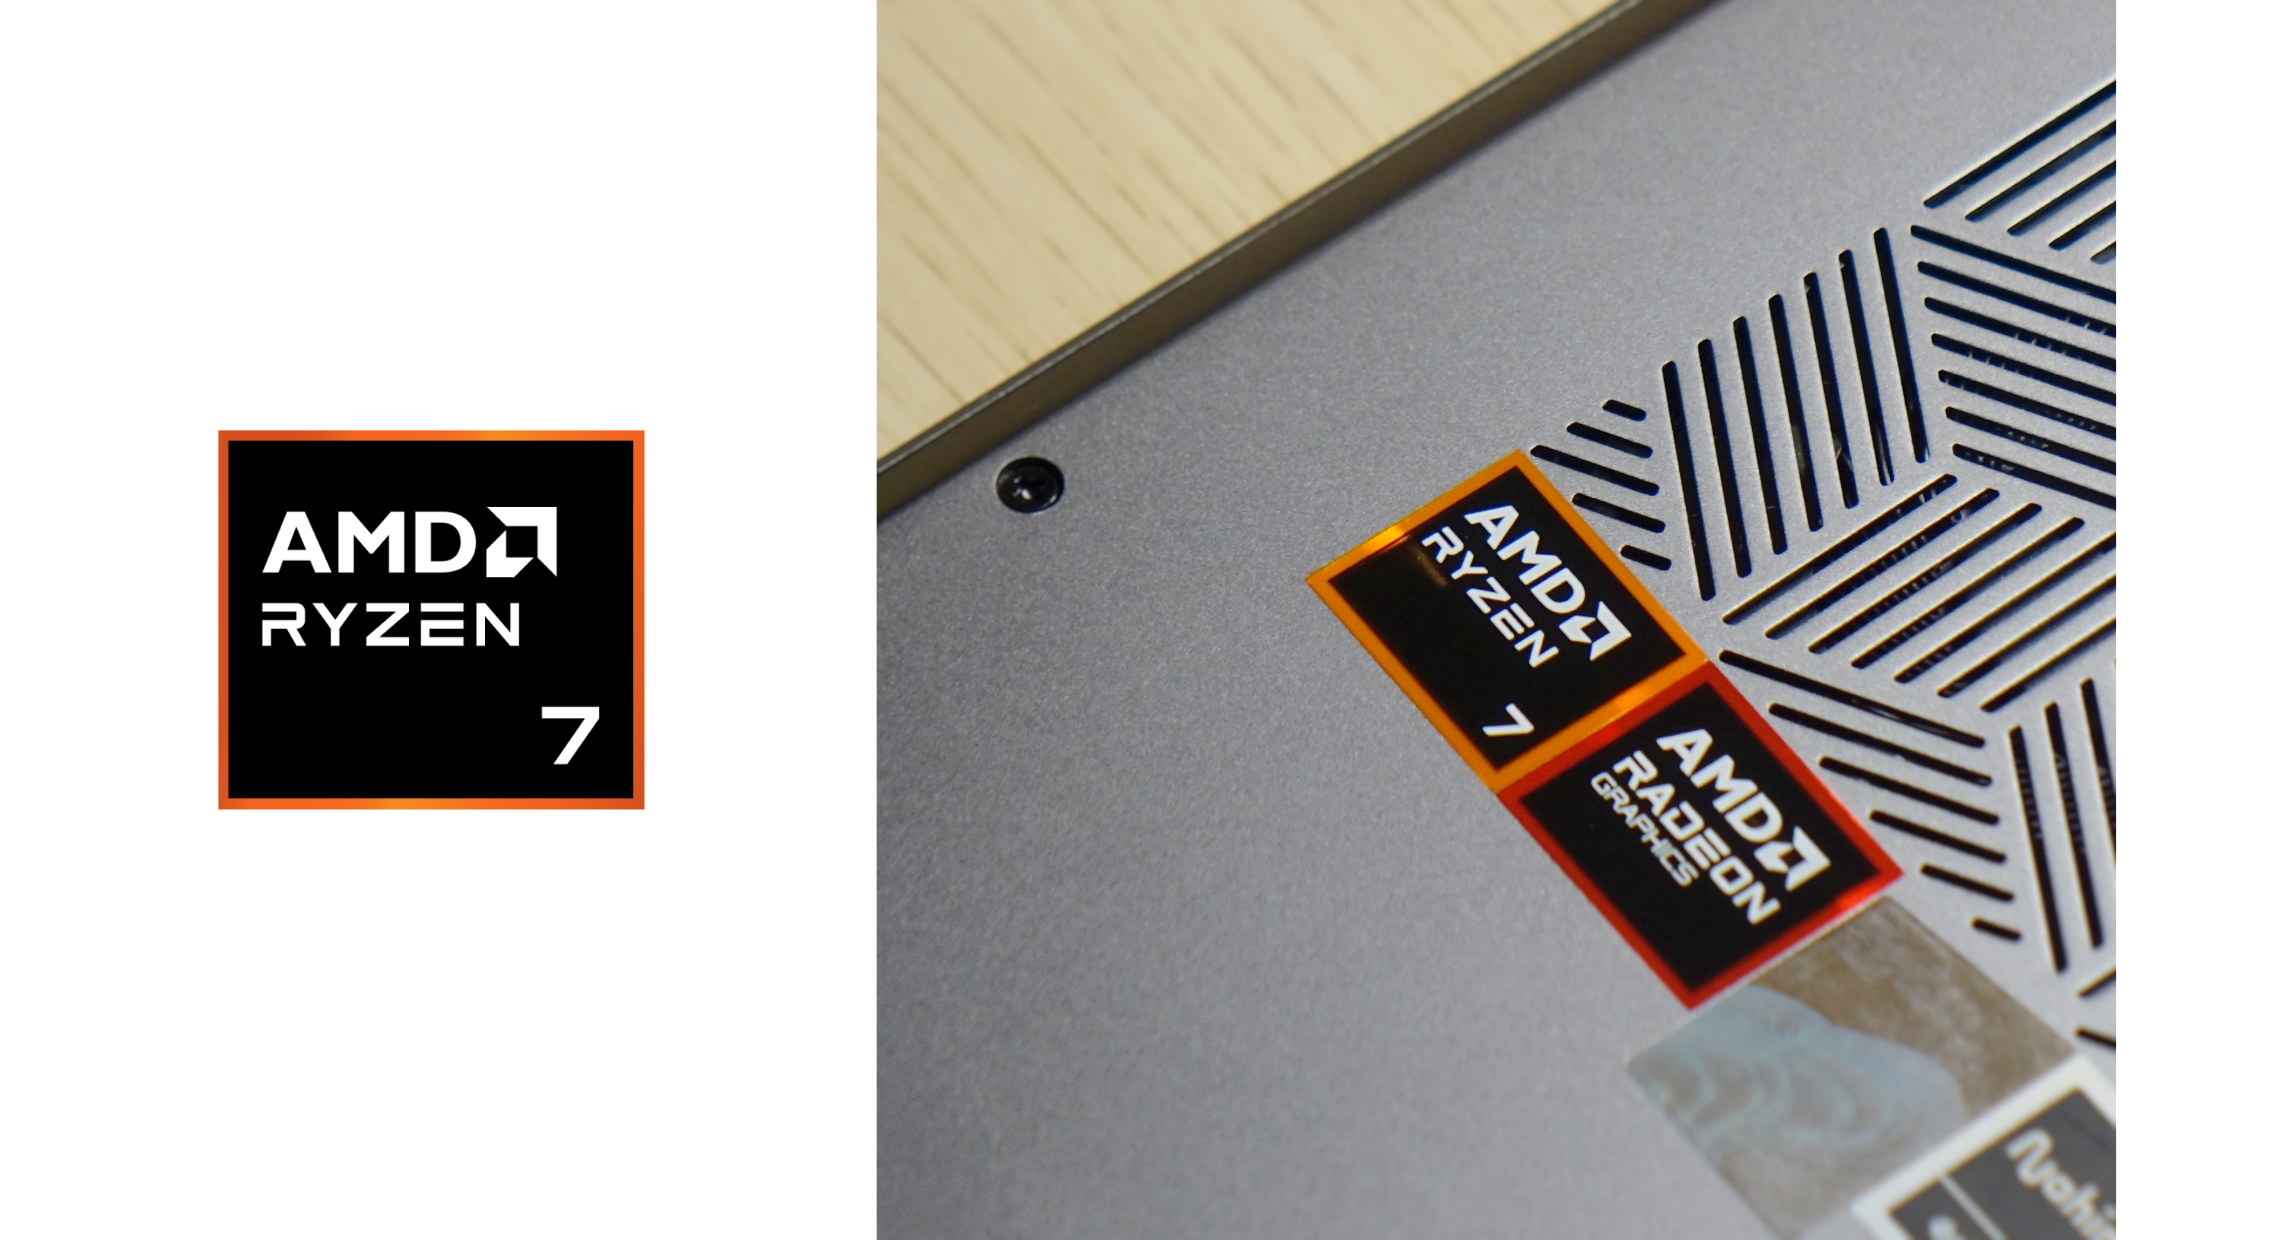
\includegraphics[width=.6\textwidth]{assets/basic/AMD_sticker.png}
      \caption{AMD的贴纸}
      \label{fig:AMD_sticker}
    \end{figure}
  \item AMD 公司现在主要的 CPU 产品线称作「锐龙」(Ryzen),而锐龙系列也分成了 3 个档次——「R5」「R7」和「R9」\footnote{其实还有 R3,但是很少在消费市场见到。}。大多数使用 AMD CPU 的电脑会粘贴类似\autoref{fig:AMD_sticker} 的橙黑或橙灰色贴纸。
\end{itemize}

\begin{note}
  除了英特尔和 AMD 之外,亦有一些厂商能够生产电脑的 CPU,例如苹果、高通,以及国产厂商龙芯、华为等。不过,这些厂商生产的 CPU 与英特尔、AMD 的 CPU 往往并不兼容,使用这些 CPU 的电脑需要使用专用的系统和软件。想了解更多有关这些 CPU 的细节?请阅读本书超越篇的\chapref{cha:program-and-arch}。
\end{note}

我们常常说一台电脑是「双核」「四核」的,这里的「双核」「四核」就是处理器中的概念。今天,几乎所有 CPU 都在芯片中安装了多个「核心」,相当于一个个协同起来的独立的小处理器。例如,「双核」意味着在一枚处理器芯片上集成了两个核心,相当于两个大脑协同工作,当我们需要用电脑同时做很多事情的时候就有所裨益。同理,「四核」「八核」就是在一个芯片上集成了四个甚至是八个核心。现在,一些 CPU 还使用「大小核」设计,混合使用大小两种规格不同的核心,来实现性能和功耗之间的平衡。下图中,左方是一枚四核 CPU 示意图,右方则是一枚采用大小核设计的六核处理器示意图(图片非实际比例)。

\begin{figure}[htb!]
  \centering
  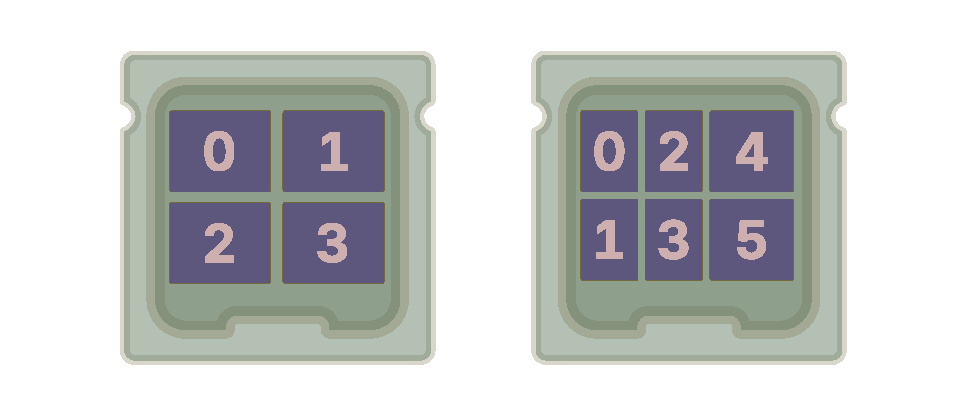
\includegraphics[width=.6\textwidth]{assets/basic/Multicore.pdf}
  \caption{多核CPU示意}
  \label{fig:Multicore}
\end{figure}

然而,核心数只能反映「脑子多不多」,但无法刻画「一个脑子有多快」。要衡量一颗 CPU 的性能,除了直观地根据厂商划定的这些低中高端系列之外,「主频」也是一个重要的参考。所谓「主频」指的是这 CPU 一秒种能够「工作」的次数,人们通常使用单位「GHz」来标注它。1 GHz 就表示「1 秒能『工作』10 亿次」。CPU 通常有一个「基准频率」和「加速频率」,前者是 CPU 正常工作时的稳定频率,后者则是在短时间内应对复杂任务时能达到的最高频率。目前,常见的台式机 CPU 的基准频率和加速频率能达到 3 GHz 和 5 GHz,而笔记本则在 2 GHz 和 4 GHz 左右。

需要强调的是,\regcolor{并不是说核心数越多、主频越高的处理器性能一定越好},更\regcolor{不是说 i7 处理器就一定比 i5 更好},也\regcolor{不是说英特尔和 AMD 有孰优孰劣之分}。我们应该综合理解这些概念:每个品牌都会随着时间推移一代代地更新,每一代都有着的不同系列,有的系列高端,有的系列低端;每个系列也都有自己的不同型号,有的型号性能强,有的型号性能弱。CPU 的性能并不与某一个因素呈线性的关系,而是多个因素叠加的结果。

\begin{figure}[htb!]
  \centering
  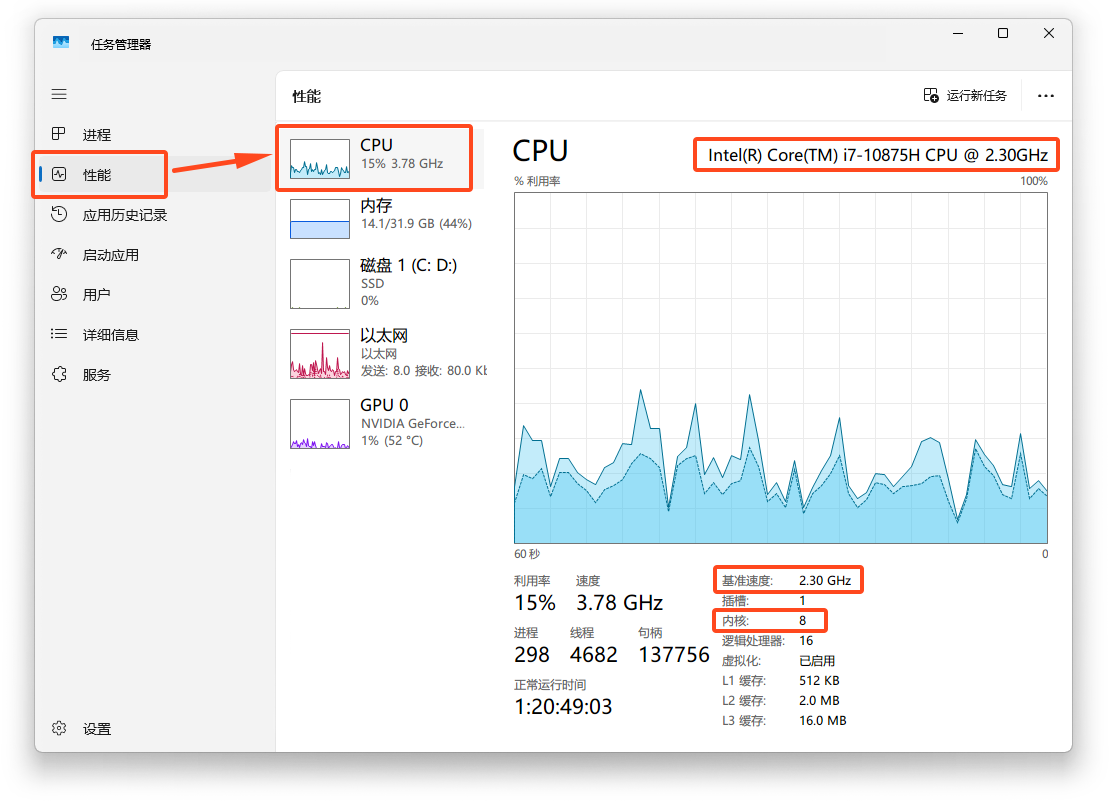
\includegraphics[width=.7\textwidth]{assets/basic/Check_CPU.png}
  \caption{在任务管理器看看CPU}
  \label{fig:Check_CPU}
\end{figure}

按 \keys{Ctrl + Shift + Esc} 打开「任务管理器」,选择【性能】页面,就能看见 CPU 的型号、基准频率(标注为【基准速度】)和核心数(标注为【内核】)。

\begin{note}
  你也可以右击【开始按钮】,选择【任务管理器】来打开「任务管理器」。
\end{note}

\subsection{内存(RAM)}

紧接着,我们介绍能直接与处理器交流的部件——内存,英文简写「RAM」。上一小节提到,处理器相当于大脑,但与大脑不同的是,处理器只能\regcolor{处理}数据,而这些待处理的数据,需要依赖外部的元件来临时存放。内存就是用来临时存放数据的。

内存的核心组件是一个个黑色的「内存芯片」。目前,内存芯片的主要生产厂商集中在韩国和中国台湾。这些芯片通常被排列在条形电路板上,形成一个模块,方便插入电脑主板进行更换或升级。这样的整体被称为「内存条」。如下图所示,左侧展示的是台式电脑使用的内存条,而右侧则是笔记本电脑使用的版本。不过,\regcolor{为了节省内部空间,很多笔记本电脑选择将内存芯片直接焊接在主板上,这种设计的内存无法更换或升级}。

\begin{figure}[htb!]
  \centering
  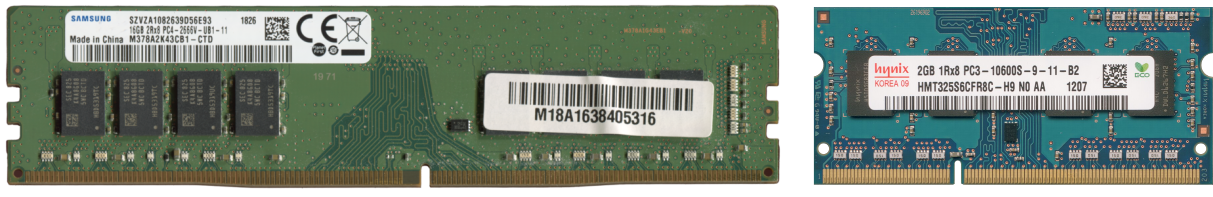
\includegraphics[width=.9\textwidth]{assets/basic/Two_memories.png}
  \caption{不同的内存条}
  \label{fig:RAMs}
\end{figure}

前文说,内存直接与处理器进行数据交流。与处理器那极快的运算速度相匹配,内存的读取与写入速度也是极快的。但内存有一个特点——\regcolor{断电即丢失数据}。也就是说,当你电脑关机,内存中的数据便不复存在,又回到白纸一块。这种特性决定着,内存只能用来在电脑工作时临时存储信息。

回到前面老师批改作业的场景。办公桌的中央区域可以理解为「内存」:老师将作业放在办公桌中央批改,是因为这里改起来最方便;处理器将数据放在内存中处理,是因为这里读取和写入速度最快。办公桌中央不能总是放着东西,不然会弄乱、弄丢;内存中的数据一旦断电就会消失,因此总是临时的。

在 21 世纪初,电脑内存的容量不大,有 512 MB 已经不得了了。但随着科技发展,现如今,大容量内存已经司空见惯。在今天,要想让一台电脑能基本流畅运行,内存容量应当至少有 8 GB。当然这东西倒是多多益善,就像更大的桌子能摆更多东西一样,\regcolor{更多的内存意味着更多的空间来让处理器存放数据,也就意味着电脑能同时处理更多的任务,基本意味着电脑更加流畅。}据我们的经验,在目前(2024 年),16 GB 的内存对于日常使用已经够用;但如果你有大型游戏、三维建模、大型软件开发等需求,选择 32 GB 乃至更大的内存会更加合适。

\begin{note}
  对应到手机中,内存有时会被手机厂商称为「运行内存」,不过我们不推荐如此称呼。原因请参见下面「硬盘」一节。
\end{note}

在任务管理器的【性能】页的【内存】一栏,你可以看见自己电脑的内存总量等信息。

\subsection{硬盘}

内存是用来临时存储数据的,而硬盘则是用来长久保存数据的。与内存相比,硬盘的读写速度要慢得多,但存在硬盘中的数据不会因为断电而轻易消失,因此,硬盘是数据的最初的起点和最终的归宿:处理器在一开始,从硬盘中取出数据放入内存,在内存中处理数据,处理完成之后,再将新的数据放回硬盘。

\begin{note}
  所以,你电脑的所有资料都存在硬盘里。想直接拿走你的资料,应该去拿硬盘,而不是拿走显示器或别的什么东西。
\end{note}

\regcolor{除了各种各样的数据——各种文档、图片、音乐——之外,电脑上各种各样的软件本身,也是存放在硬盘里面的。}相信你在手机上有过这样的经验——手机的「存储空间」不够用,除了删掉一些不需要的照片、视频外,卸载不常用的 app 也是一个快捷的办法。在电脑上,情况是一样的:卸载软件,释放的其实就是硬盘上的空间。

\begin{figure}[htb!]
  \centering
  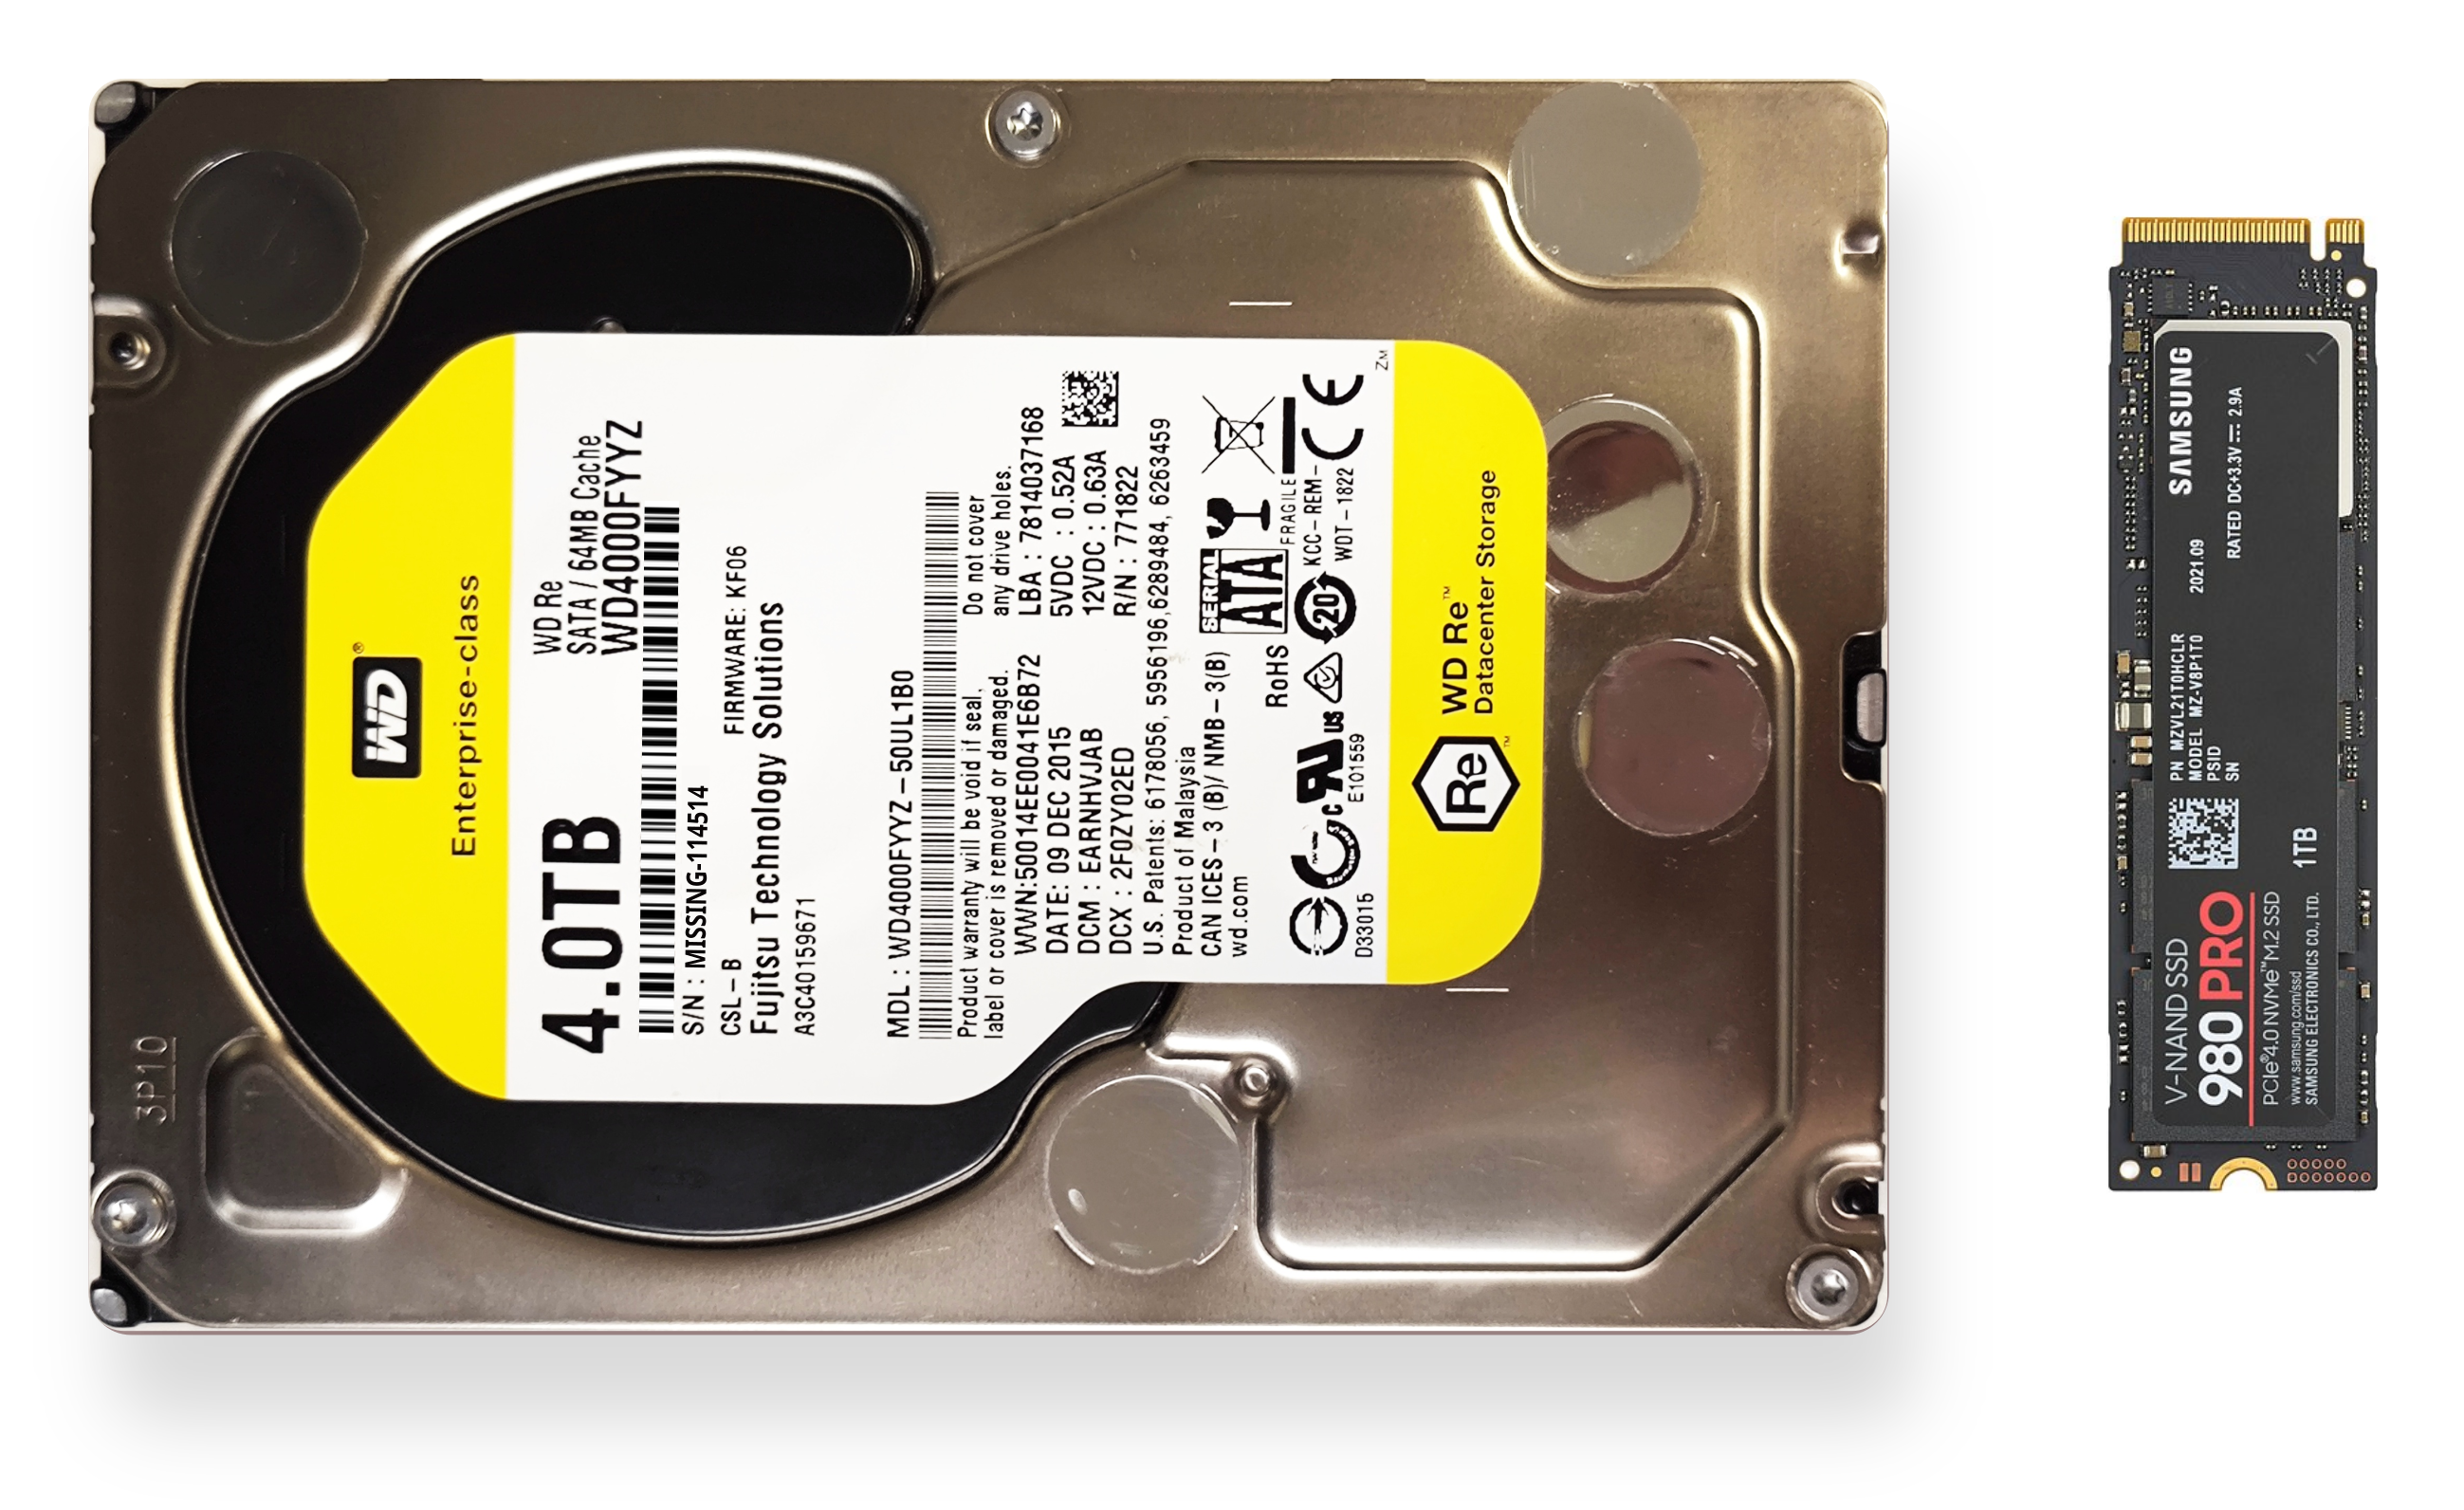
\includegraphics[width=.7\textwidth]{assets/basic/HDD_and_SSD.png}
  \caption{常见的硬盘}
  \label{fig:HDD_and_SSD}
\end{figure}

在前面老师批改作业的场景当中,办公桌两侧堆作业的地方可以理解为「硬盘」:大量的作业被堆在那里,整齐摆放,不会弄散、弄丢,但老师总是要把作业取到趁手的地方(办公桌中央)来批改;大量的数据被存在硬盘里,不会因为断电就丢失,但处理器总是要把数据放在快速的地方(内存)来处理。

简单来说,硬盘现在分为两种,一种叫「机械硬盘」(Hard Disk Drive,简称「HDD」),如\autoref{fig:HDD_and_SSD} 左侧所示,容量大、价格低、速度更慢,利用电磁原理存储数据。另一种叫「固态硬盘」(Solid State Drive,简称「SSD」),如\autoref{fig:HDD_and_SSD} 右侧所示,容量小、价格高、速度较快(但远远没有内存那么快)。SSD 用芯片存储数据,但这种芯片和内存的那种不同,断电还能保持数据。不过,不管是哪种硬盘,如果硬盘许久不用(不给它通电),那里面的数据也会慢慢消失,固态硬盘大约是 3 至 5 年,而机械硬盘最多 20 年——所以,对于存了东西但没有装入电脑的备用硬盘,要定期拿出来通电运转一下。

在今天(2024 年),标称容量 1 TB 的固态硬盘大约 500 元,机械硬盘大约 300 元;标称容量 2 TB 的固态硬盘大约 800 元,机械硬盘大约 400 元。因此,有些电脑会用一块小容量(512 GB 及以下)的固态硬盘,搭配一块大容量(1 TB 及以上)的机械硬盘来实现各自功能的互补。但也有一些中高端电脑会直接选用一整块大容量(比如 1 TB 甚至 2 TB)的固态硬盘而不再使用机械硬盘。

\regcolor{一块硬盘的空间可以被划分成不同的「盘」(学名叫「分区」)来更好地使用}。双击桌面上的【此电脑】来打开「文件资源管理器」,你看到的「C 盘」「D 盘」就是各个分区。在下一章\chapref{cha:file-and-file-management},我们将向你介绍如何管理好自己硬盘上的东西。 

\begin{figure}[htb!]
  \centering
  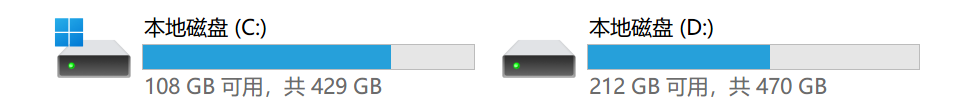
\includegraphics[width=.8\textwidth]{assets/basic/Partitions.png}
  \caption{一些分区}
  \label{fig:partitions}
\end{figure}

\begin{note}
  如果你在桌面上没有看到【此电脑】图标,你也可以按下 \keys{\Windows + E} 组合键来打开文件资源管理器,然后在左侧的导航栏中找到【此电脑】。

  如果你想在桌面上显示【此电脑】图标,请先打开系统设置,然后选择【个性化】,找到【主题】。

  \begin{center}
    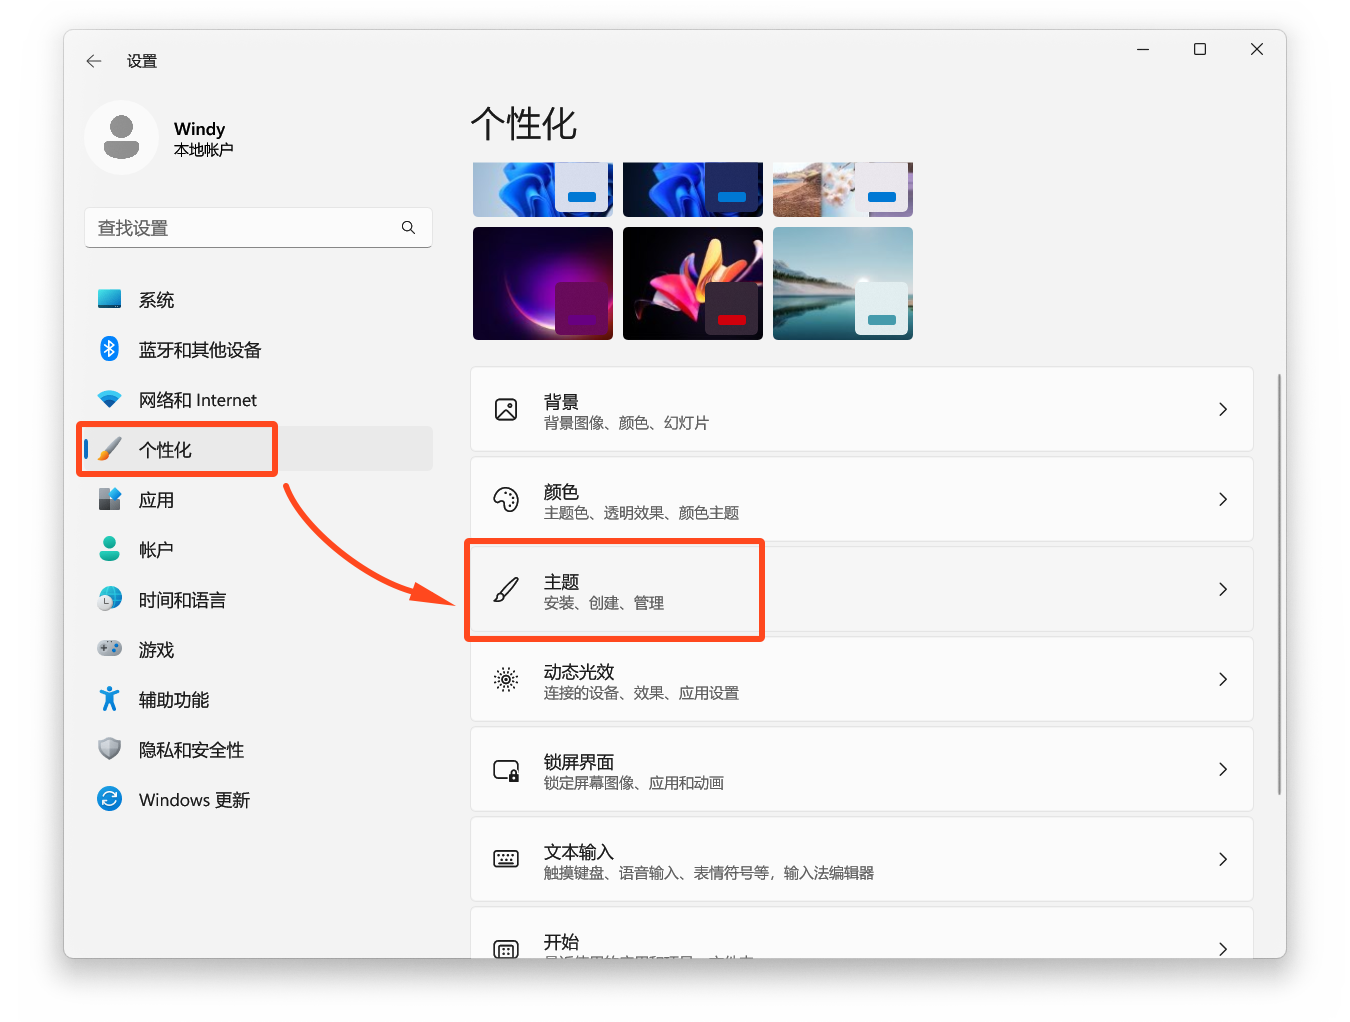
\includegraphics[width=.8\textwidth]{assets/basic/Open_personalization_in_settings.png}
    \captionof{figure}{找到【主题】设置}
    \label{fig:Open_personalization_in_settings}
  \end{center}

  然后,在界面下方找到【桌面图标设置】(Windows 10 可能显示在界面右方),勾选【计算机】(即【此电脑】),再点击【应用】。你也可以把其他几个常用的图标勾选上,比如【用户文件】、【回收站】等。

  \begin{center}
    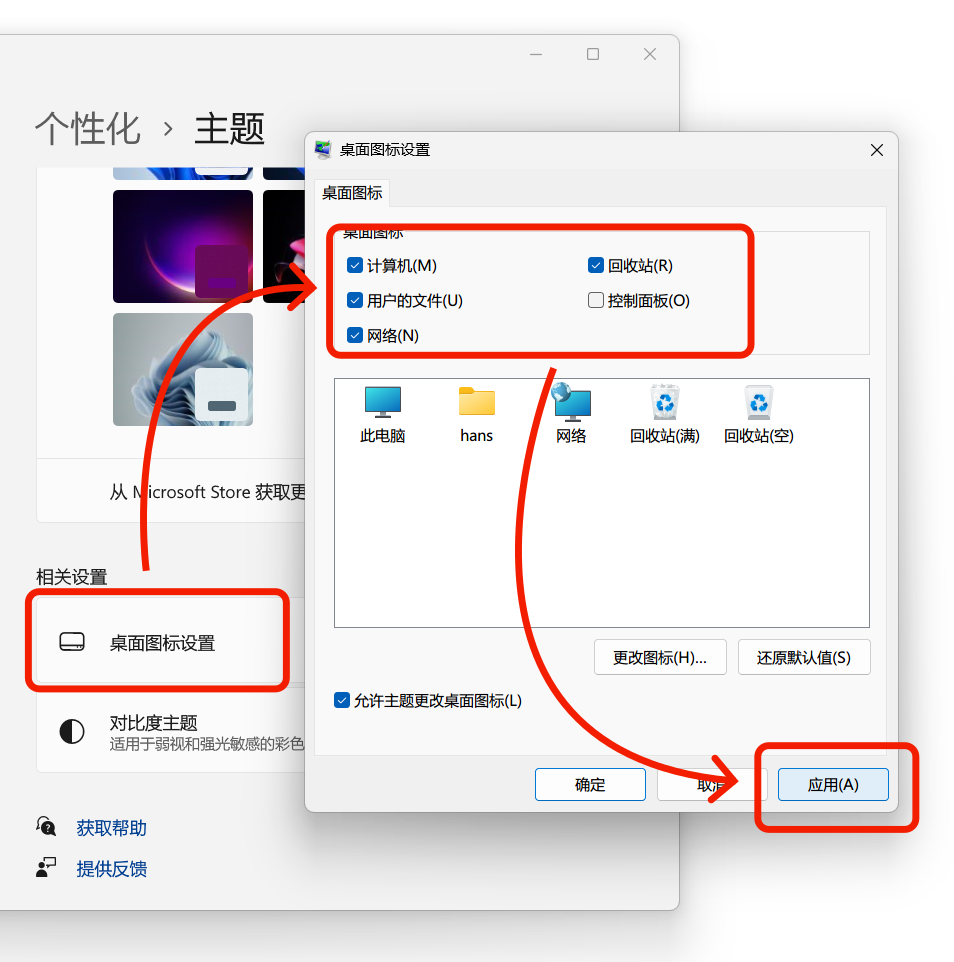
\includegraphics[width=.65\textwidth]{assets/basic/Select_This_PC.png}
    \captionof{figure}{选择要显示的图标}
    \label{fig:Select_This_PC}
  \end{center}

  这样,你的桌面上就会显示那些对应的图标了。
\end{note}

\regcolor{硬盘对电脑使用体验的影响,主要是打开软件的速度,包括开机的速度。}这是很容易理解的,因为数据和软件本身原先都是存在硬盘里的,处理器从硬盘里取数据的速度就直接影响着软件启动或者说加载的时间。

\begin{note}
  手机中用类似固态硬盘一样的芯片来存储数据,有些手机厂商和商家会称之为「内置存储」「存储内存」甚至是「内存」,但它\regcolor{完全不是}内存。这是为什么有人会弄混内存和硬盘的根源之一。人们常说的「手机内存不够」,指的往往是存储空间(可以称「手机的硬盘」)不够,而不是真正的「内存不够」。
\end{note}

\begin{figure}[htb!]
  \centering
  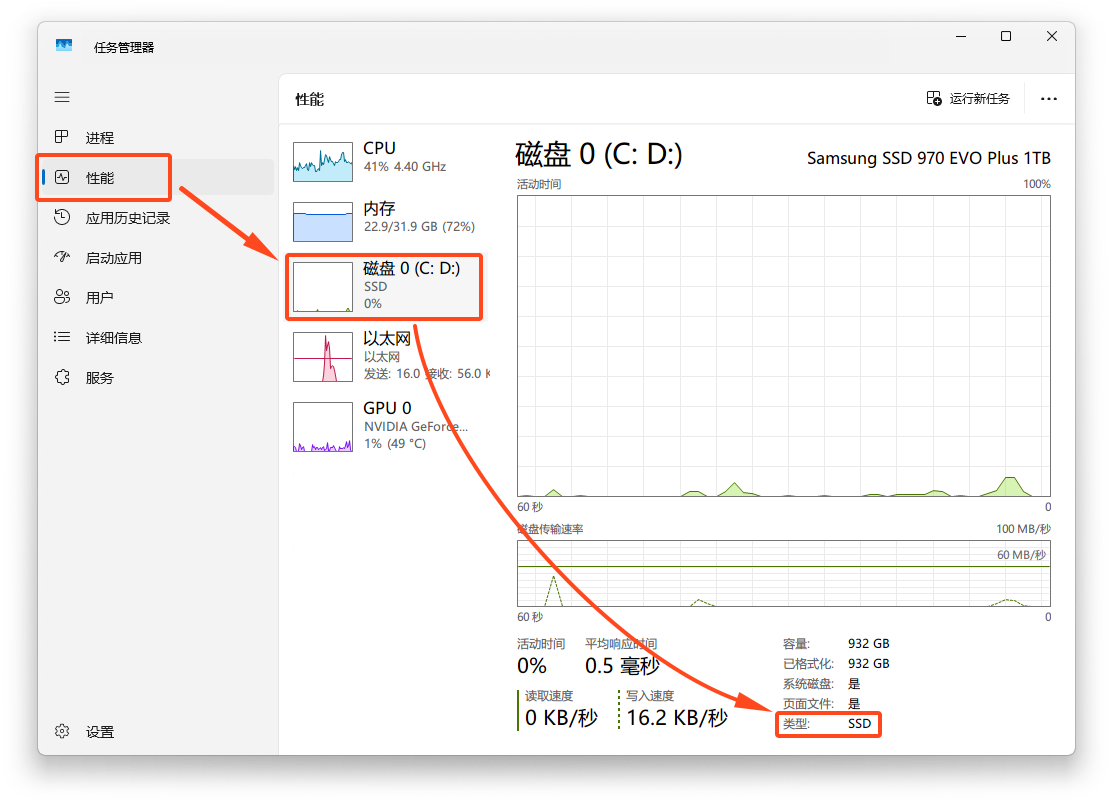
\includegraphics[width=.65\textwidth]{assets/basic/Check_disk_status.png}
  \caption{在任务管理器看看硬盘}
  \label{fig:Check_disk_status}
\end{figure}

打开「任务管理器」,切换到【性能】选项卡,其中【磁盘 0】【磁盘 1】就是一块块硬盘,其后的括号内则列出了该硬盘上的分区。点击一块硬盘,可以看到它的大小和类型(机械硬盘 HDD、固态硬盘 SSD)等信息。

\subsection{显卡(GPU)}

如果你是喜欢玩游戏的读者,「显卡」将是你在选购电脑时需要着重考虑的一个因素。

以前,「显卡」就是电脑里面的一个独立的模块,像一张卡一样插接在主板上。这个模块的功能是专门进行画面的绘制和图像的处理,因而得名「显卡」。所有显示在屏幕上的画面,都是由显卡绘制的。因而,\regcolor{显卡的好坏对游戏和图形相关的工作(比如三维制图、视频编辑)有较大影响}。\autoref{fig:GPU_parts} 展示了一块老旧的电脑显卡,其中 ➊ 是用于连接显示器的端口,➋ 处则是与电脑主板连接的触点。➌ 为这块显卡的散热风扇,而在其下方压着的 ➍,就是显卡的核心部分——图形处理器(Graphics Processing Unit,简称 GPU)。

\begin{figure}[htb!]
  \centering
  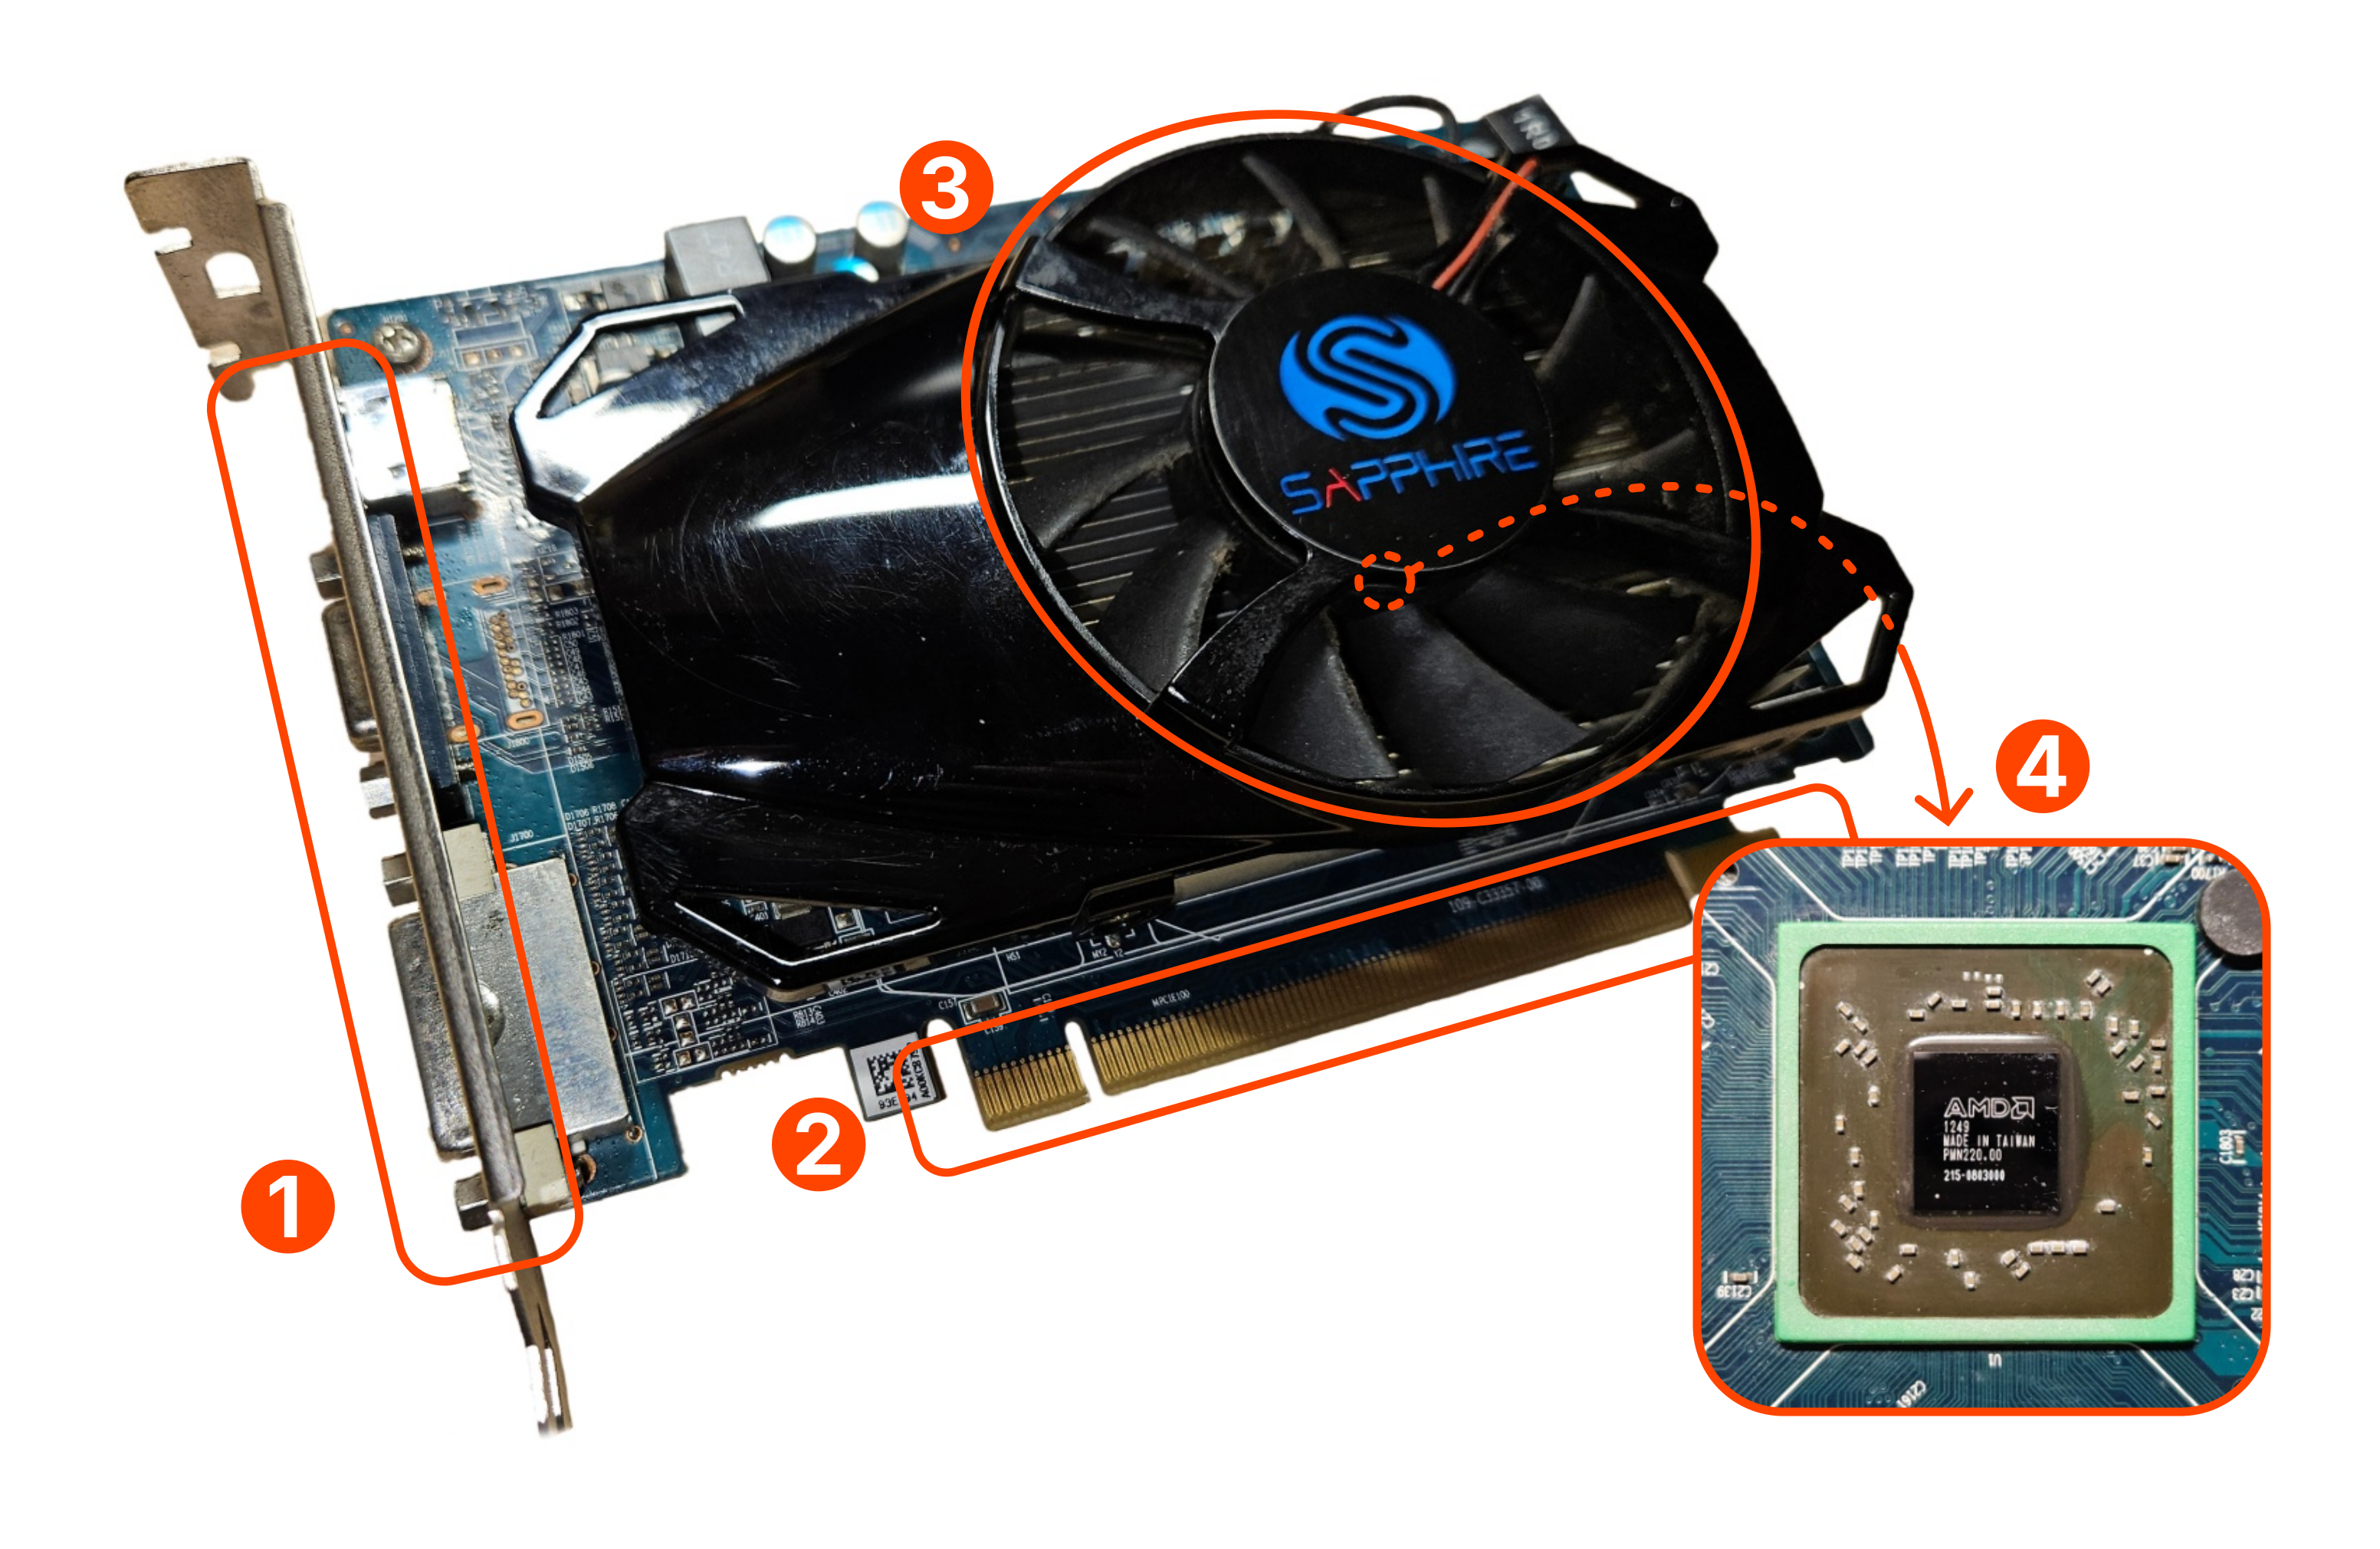
\includegraphics[width=8cm]{assets/basic/GPU_parts.png}
  \caption{老显卡(也是现在显卡)的各部分}
  \label{fig:GPU_parts}
\end{figure}

\begin{note}
  也就是说,GPU 是一枚芯片,而显卡是承载着这个芯片的模块。不过现在,人们习惯于将这两个词混用——既可以用「GPU」代指整个显卡,也可以用「显卡」或「显卡芯片」一词来特指 GPU 那枚芯片。强求区分它们显得有点古板学究气了,因此在本书中,我们也会混合使用两种称呼。
\end{note}

为什么上面那段要加上「以前」两个字呢?因为随着半导体技术的发展,人们后来发现,GPU 可以「集成」到处理器\footnote{一开始,集成显卡并不是集成到处理器中的,而是集成在主板上的一个芯片之中(称为「北桥」),后来才集成到了处理器里面。}中,换言之,就像多核处理器把几个核心放在一个芯片上一样,GPU 也可以和 CPU 做成一块芯片。容易想到,这样集成到一起之后,受限于芯片整体的大小,GPU 不能做得性能很强了:CPU 就在它边上,与它一起发热,一起分享能量。但是,通过这种方式,可以有效缩小硬件的体积,也能降低功耗。因而,发展到今天,GPU 在电脑中的形态有了以下两种:

\begin{itemize}
  \item \regcolor{集成显卡},简称「\regcolor{集显}」,又称「\regcolor{核显}」,英特尔称「核芯显卡」,AMD 则将 GPU 和 CPU 构成的整体一同称为「APU」。GPU 被安排在处理器的同一片芯片上,性能相对较差,能应付大多数工作,但游戏、制图等特定工作就不太行了。集成显卡功耗很低,而且省去了用户单独购买显卡的麻烦。
  \item \regcolor{独立显卡},简称「\regcolor{独显}」。GPU 仍然是一片独立的芯片,以显卡模块的形式安装在电脑内。这样的 GPU 性能较强,但换来的是更高的功耗、更大的体积和更多的发热等。如果你喜欢玩游戏(尤其是大型 3D 游戏),又或者从事视频编辑、三维设计等工作,那么一台装有独立显卡的电脑可能是你的刚需。
\end{itemize}

今天,全世界生产\regcolor{独立显卡}的厂商主要有两家,一家叫「英伟达」(NVIDIA),它旗下的显卡俗称「N 卡」;另一家则是前文提到过的 AMD,它推出的显卡俗称「A 卡」。如果你有涉足过游戏交流圈,玩家所说的「RTX 4090」「GTX 1080 Ti」等都是英伟达显卡的型号,而「RX 6800 XT」「RX 580」等都是 AMD 显卡的型号。下图是英伟达网站上出售的\CJKsout*{《黑神话·悟空》联名款的} RTX 4070 Super 高端显卡,可以看到显卡上有三个大尺寸的散热风扇,这从侧面说明其功耗之大、发热之多。

\begin{figure}[htb!]
  \centering
  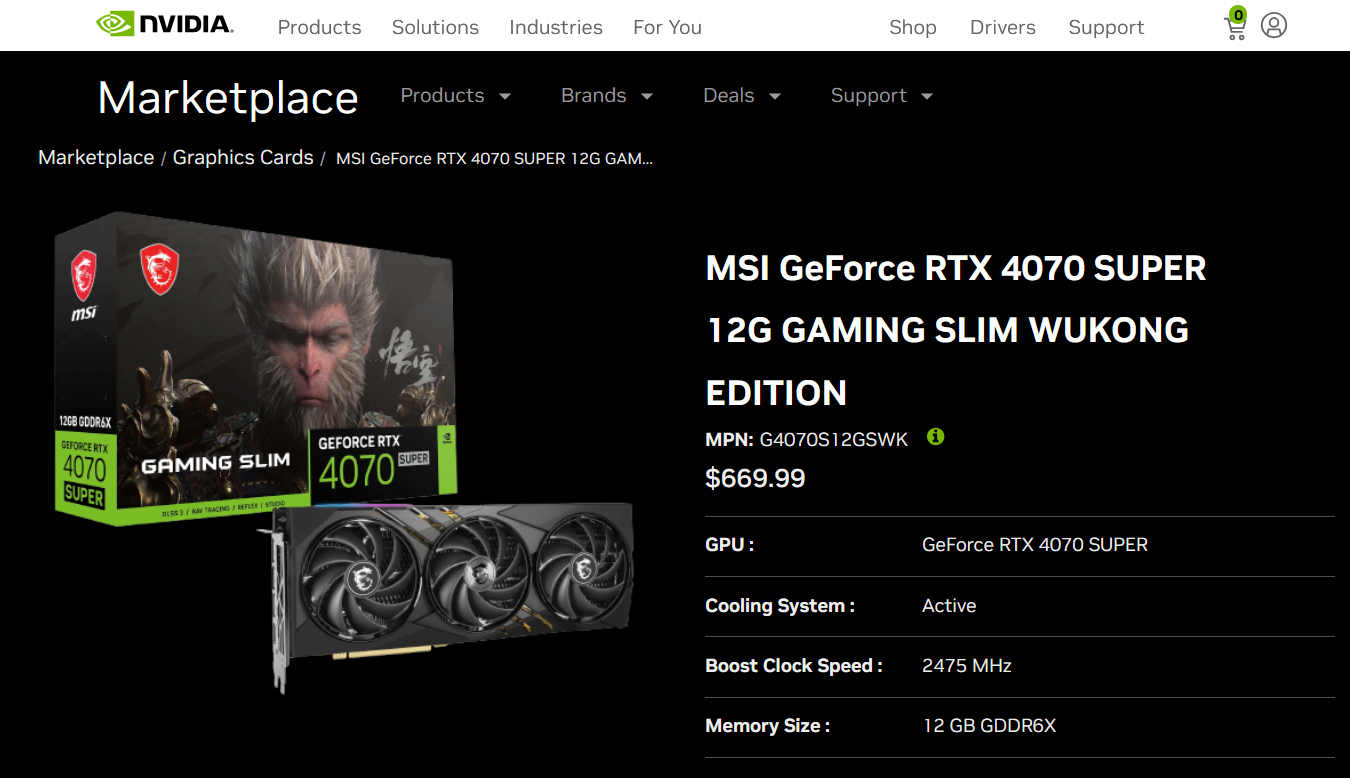
\includegraphics[width=.6\textwidth]{assets/basic/4070_storepage.png}
  \caption{在售的RTX 4070 Super}
  \label{fig:4070_storepage}
\end{figure}

\begin{note}
  除了英伟达和 AMD 之外,市面上也有一些其他品牌的独立显卡。或许来源于在集成显卡设计上的经验,英特尔也推出了自己的独立显卡系列。同时,我国公司「摩尔线程」也率先推出了面向民用市场的国产显卡,具有比较优秀的理论性能。然而,由于市面上的游戏、软件大都主要针对英伟达和 AMD 显卡进行设计、优化,摩尔线程显卡的实际体验目前还有许多的提升空间。
\end{note}

一般来说,对于笔记本电脑,轻薄本大都使用集成显卡,而游戏本大都装配有独立显卡。显然,这是由它们的使用场景和目标人群不同所决定的。不过,因为笔记本电脑内部空间相当有限,笔记本内即使装配了独立显卡,它们的性能也要比同级别的台式机独立显卡要差。同时,笔记本的独立显卡往往不是「插」而是「焊」在主板上的,我们几乎不可能对它们进行更换、升级,更别说给没有独立显卡的笔记本电脑加装一块独显\footnote{不过,如果你的笔记本电脑配有「雷电 3」「雷电 4」或「OCuLink」等接口,你可以通过这个接口连接外置的独立显卡来使用,但是这样做并不十分方便,受众并不多。}。

我们可以把 GPU 的任务理解成「根据 CPU 的命令,画出图形并输出到显示器上」。为了完成这个任务,\regcolor{GPU 拥有属于自己的内存,称为「显存」}。GPU 使用显存空间来暂时存放它正在绘制的画面,同时还要存放大量与图形有关的其他内容。这使得显存的大小成为了决定(独立)显卡性能和价格的一个重要因素。目前,高端的独立显卡拥有 10 GB 甚至 20 GB 以上的显存,这使得它们得以从容应对各种复杂的游戏画面。而至于集成显卡,它们则需要从电脑内存中「借」一部分空间充当显存,因此更难以应付大量的图形工作。

值得注意的是,近些年来,随着人工智能(AI)技术的发展,GPU 的功能已经不再局限于「打游戏」「制图」等图形工作——\regcolor{在 AI 模型的训练和推理过程中,GPU 的并行计算能力能提供比处理器更好的性能},同时独立显卡的显存还能提供比电脑内存更快的访问速度。如果你了解过 AI 绘画或 AI 作曲等技术,在它们的说明文档中,你一定会看到对 GPU 的需求。若你对这方面有兴趣,那么 GPU 的性能,尤其是显存的大小,就成了你选购电脑时的重要考虑因素。

\begin{note}
  想了解和 AI 有关的更多知识?没问题!请看超越篇的\chapref{cha:bring-intelligence-to-machines}。
\end{note}

在任务管理器中,我们同样可以看到有关显卡的信息:在【性能】页面左侧的列表末尾,【GPU 0】【GPU 1】等就表示着我们电脑上的一张张显卡。

\section{与我们「打交道」的软件}

\subsection{软件与操作系统}

由处理器、内存、硬盘以及各种各样的外围电子元件,共同构成了一台电脑的硬件部分。而在硬件之上,具体的工作任务是由软件来指派的。

我们可以用每天都在用的手机来理解:\regcolor{手机上,无论是我们自己安装的「QQ」「微信」「网易云音乐」,还是手机预置的「电话」「短信」,都属于「软件」}。「QQ」「微信」指挥硬件去利用网络收发信息,利用屏幕展示数据;「网易云音乐」指挥硬件去播放声音,同时在屏幕上展示评论;「电话」「短信」指挥硬件利用无线电模块发送和接收信号……同样一部手机,硬件还是那个硬件,但能通过不同的软件行使不同的具体功能。

而在「QQ」「微信」「电话」等 app 和纯粹的硬件之间,有\regcolor{一个更大,而且更「底层」的软件,称为「操作系统」}。简单地说,操作系统「夹」在各软件和硬件之间,为软件具体行使功能提供了一系列方便的「接口」。有了操作系统,网易云音乐 app 不再需要真正地去想「怎么让喇叭发声」,而只需要考虑「怎么告诉操作系统让喇叭发声」。「让喇叭发声」是一个带些复杂物理知识的过程,但「告诉操作系统让喇叭发声」则相对简单得多。

\begin{figure}[htb!]
  \centering
  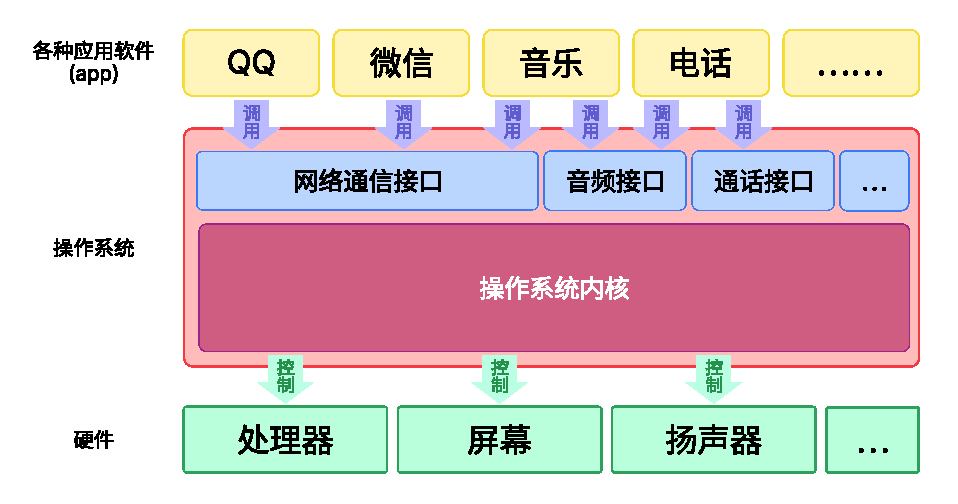
\includegraphics[width=.75\textwidth]{assets/basic/OS_structure.pdf}
  \caption{App、操作系统和硬件的关系}
  \label{fig:OS_structure}
\end{figure}

\begin{note}
  尽管操作系统是一个特殊的软件,但在日常生活中,「软件」一词通常只指微信、QQ 或是 Word、PowerPoint 等「应用软件」,即 app。在本书中,除非特别说明,「软件」和「app」是相同的含义,我们会混合使用它们。
\end{note}

由于上层的软件需要依赖操作系统来实现功能,而每个操作系统留给软件的接口细节上也有所不同,因此,\regcolor{针对不同操作系统开发的软件是不能直接通用的}。软件厂商一般会为不同的操作系统开发同一款软件,这样就能照顾到使用不同系统的用户。

今天,主流的手机操作系统有「安卓」(Android)、「iOS」以及「鸿蒙」(Harmony OS)。安卓系统是开放的,因此被各个手机厂商广泛使用,而 iOS 和鸿蒙目前则分别用在苹果和华为的设备上。如果你在网上下载过手机 app,一定会注意到厂商要根据操作系统提供不同的下载入口,这正是因为不同系统上的软件相互不兼容。

\begin{figure}[htb!]
  \centering
  \includegraphics[width=.8\textwidth]{assets/basic/Three_systems.pdf}
  \caption{三大主流电脑操作系统}
  \label{fig:Three_systems}
\end{figure}

而在电脑上,「Windows」「Linux」及「macOS」是最常见的三种操作系统。\regcolor{Windows 最为普遍,几乎所有的个人电脑都运行着 Windows 系统}。Linux 是一种开源的操作系统,主要在服务器上使用,一些专业人士也会在日常使用。此外,近年来,一些机关和事业单位也开始使用基于 Linux 的国产操作系统(如统信 UOS、银河麒麟等)以保障国家信息安全。macOS 则是苹果推出的电脑操作系统,理论上只能用于苹果的电脑。\autoref{fig:Three_systems} 中,(a) 至 (c) 依次是 Windows 11、Linux(使用 GNOME 桌面环境)和 macOS Sonoma 的界面。

\subsection{Windows 操作系统}

我们绝大多数人都在使用 Windows 操作系统,《你缺计课》亦是一套基于 Windows 的电脑教程。所谓「Windows XP」「Windows 7」和「Windows 10」则是 Windows 操作系统的不同版本。

Windows 由美国的微软公司所开发,诞生于 1985 年。到今天(2024 年),Windows 已经经历了数个大版本的更新\footnote{关于 Windows 的一点点更新历史,可以参见\chapref{cha:recover-from-bsod}一章。}。今天,除了苹果以外几乎所有品牌的个人电脑都运行着 Windows 系统。目前最新的 Windows 版本是 Windows 11(发布于 2021 年 10 月 5 日),它与 Windows 10(发布于 2015 年 7 月 29 日)一同占领了大部分电脑。在有些地方,一些稍旧的计算机运行着 Windows 7,而更老的 Windows 版本(如 Windows XP)目前已经鲜有使用。不同版本 Windows 系统之间会有操作细节、使用体验上的不同,不过往往最直观的不同是它们的外观。下图中,(a) 和 (b) 分别展示了 Windows 11 和 Windows 10 的界面。

\begin{figure}[htb!]
  \centering
  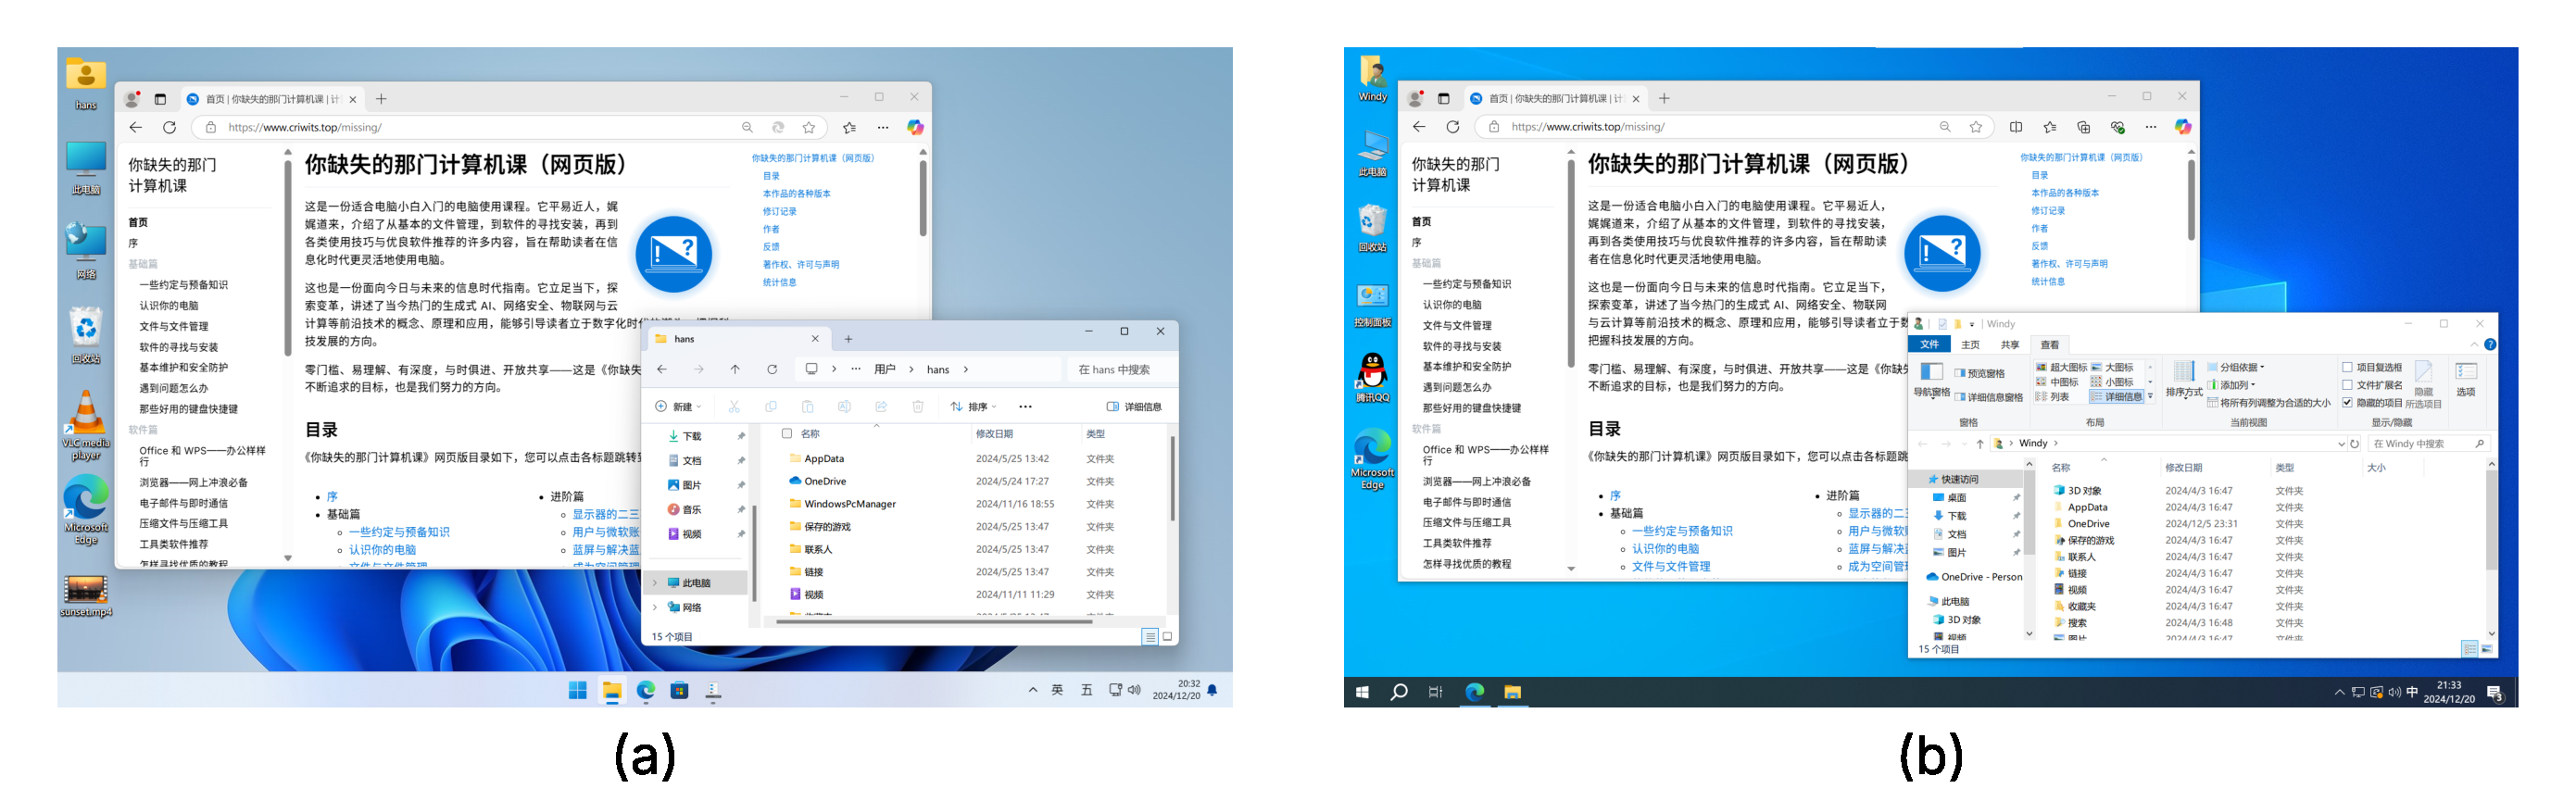
\includegraphics[width=.9\textwidth]{assets/basic/Win_11_and_10.pdf}
  \caption{如今的两大Windows}
  \label{fig:Win_11_and_10}
\end{figure}

\begin{figure}[htb!]
  \centering
  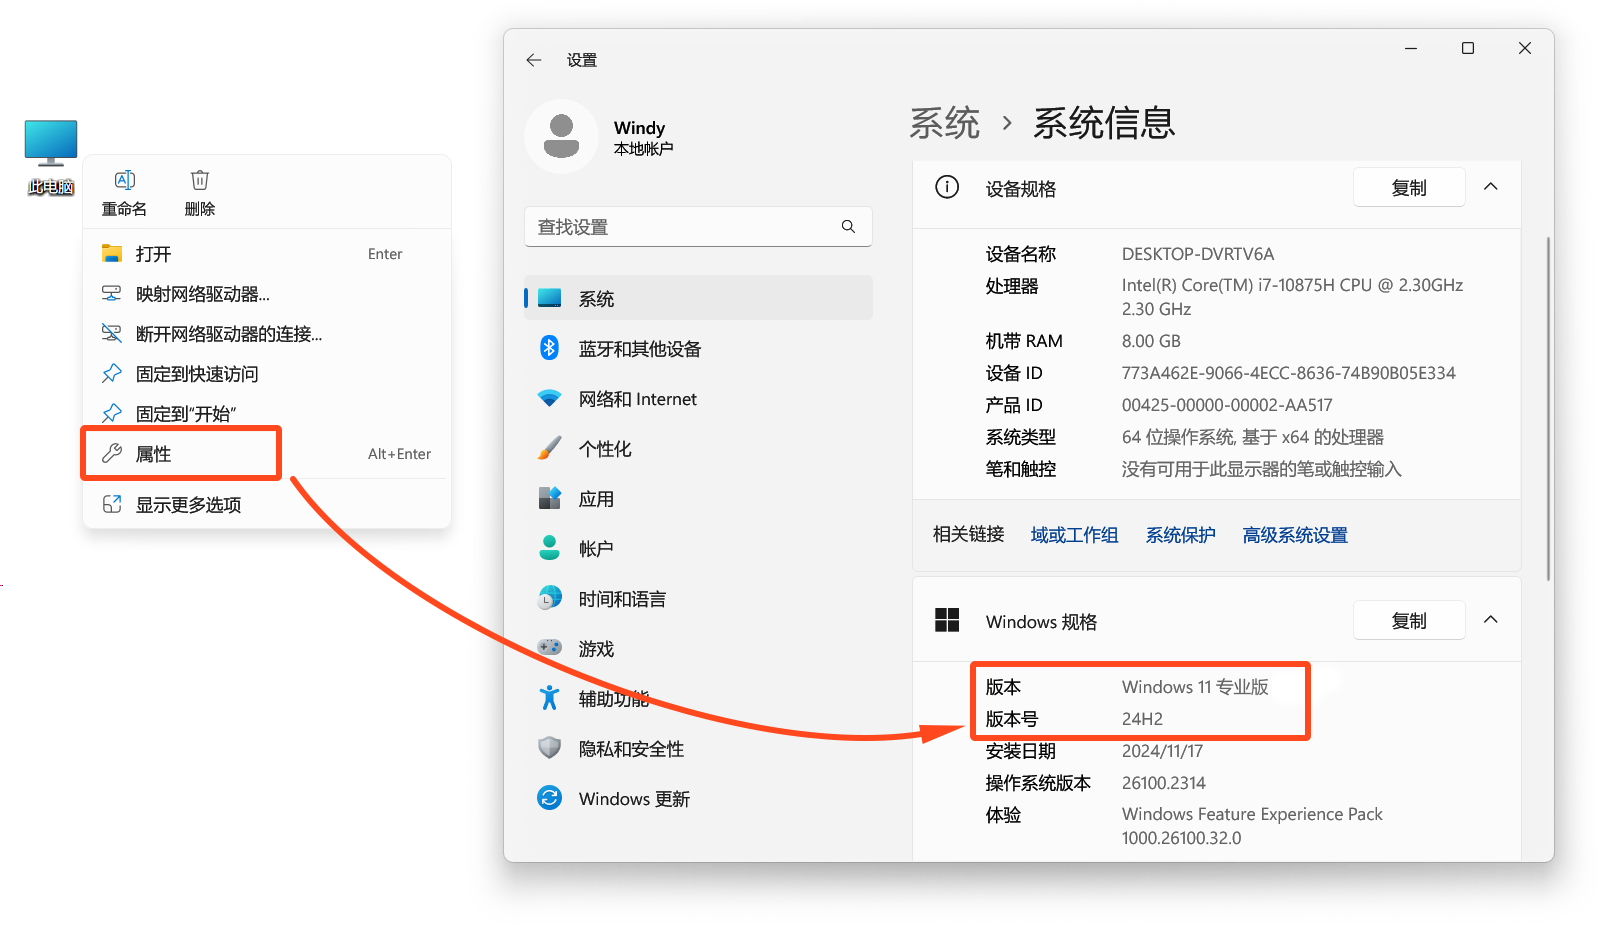
\includegraphics[width=.7\textwidth]{assets/basic/Check_Windows_version.png}
  \caption{检查 Windows 系统版本}
  \label{fig:check-windows-version}
\end{figure}

通过右键桌面上的【此电脑】并点选【属性】,或打开系统设置,选择【系统】→【系统信息】(Windows 10 则是【关于】),你可以看到自己电脑 Windows 系统的版本。

\regcolor{本书假定读者使用的系统是 Windows 11 或者 Windows 10,其中所有的操作都是基于 Windows 11 或者 Windows 10 简体中文版系统来描述的。}不过,本书所介绍的知识是通用的,如果你使用的是 Windows 7、Windows 8 或者 Windows 8.1,本书提到的多数操作你也能正常使用。一些明确仅能用于 Windows 10 和/或 Windows 11 的操作和技巧一般会特别标注。

\practice

\begin{enumerate}
  \item 通过任务管理器和【此电脑】→【属性】,查看自己电脑的 Windows 版本、CPU 型号和核心数、内存大小、硬盘大小和类型、显卡大小和类型。
  \item 你使用的是游戏本还是轻薄本?亦或是介于二者之间的所谓「全能本」?尝试翻到笔记本的底面,上网搜索它底面所写的型号,了解关于你自己机器的更多信息。
  \item 你对「电路」的认知有多少?你是否好奇 CPU 是怎么运作的?从开关、导线、电池、灯泡组成的最简单「电路」到几乎无所不能「电脑」之间到底发生了什么奇妙的变化?在本书超越篇的 \chapref{cha:program-and-arch}一章中,我们会简要向你进一步介绍这些问题。但限于《你缺计课》篇幅,我们是没法完全告诉你这些的。但是,你若有兴趣,可以去学习「电路电子技术」「计算机体系结构」「计算光刻」「纳米测量技术」等相关内容。近年来,国际形势风云变幻,我国在芯片领域仍然存在许多短板。我们希望越来越多的有志青年能投身于包括但不限于体系结构、硬件组成、数字电路乃至微电子、集成电路制造、半导体材料等领域,为我国芯片行业「补上短板」贡献自己的力量。
\end{enumerate}
